\subsubsection{Aislamiento de los SIS}


El propósito del SAL/T es permitir el movimiento de la formación de una manera segura ante una activación de las interrupciones de los SIS. Para eso, se produce una interacción con los sistemas instrumentados de seguridad en la medición del estado impuesto por los propios SIS, pero también en una imposición de estado por parte del SAL/T. La llave interruptora de los SIS se abre ante una falla o detección de condición insegura en ese SIS. En el caso de ingresar al modo aislado limitado, el sistema va a utilizar las mediciones de estado de cada uno de los SIS y aislar el que esté interrumpiendo la línea; de esta manera, la línea mantiene la continuidad, y el resto de los SIS sigue teniendo la capacidad de interrumpir las señales críticas. Además, cuando se ingresa en modo aislado total o en modo intermitente por comando remoto, o en modo parada total o en modo coche deriva, el SAL/T va a interrumpir las líneas de las señales críticas dejando sin efecto el estado de los SIS. \\    

Para realizar el aislamiento de un SIS, se conectaron las mismas terminales donde se mide el estado del SIS a un relé. Su estado normal es abierto, por lo que no afecta el estado del SIS. Sin embargo, cuando se activa la señal de control del relé por algunos de los motivos mencionados anteriormente, se conectan las señales positiva y negativa de la llave del SIS, forzando un estado de continuidad en la línea. \\ 

Para el relé de aislamiento, se eligió el modelo JW2SN-DC5V de Panasonic Industrial Devices \cite{JW2SN-DC5V}. Este es un relé de potencia que se activa con 5 V en las entradas de control y que cuenta con un arreglo de contacto de 2 salidas tipo C conocido como DPDT (\textit{double-pole double-throw}). En condiciones normales, tiene un consumo de 106 mA al activarse, ya que la resistencia de la bobina interna es de 47 $\Omega$. \\

Se eligió este modelo porque funciona como exacto reemplazo de un relé de seguridad de las mismas características de encapsulamiento y contactos como el V23047A1005A501 de TE Connectivity \cite{V23047A1005A501}. Estos relés de seguridad también son DPDT y activan con 5 VDC. Los relés de seguridad o también conocidos como relé de contactos guiados forzados tienen una configuración y técnica constructiva que cumplen con la norma EN 61810-3 \cite{norma_61810}. Estos relés tienen al menos un par de contactos normal cerrado y otro par normal abierto que están vinculados de manera mecanica lo que hace imposible que ambos estén en contacto simultáneamente; incluso en caso de falla. En la figura \ref{fig:rele_seguridad} se observa el funcionamiento de un relé de seguridad. Este tipo de relé es recomendado para aplicaciones en sistemas críticos porque permite utilizar el contacto primario como actuador, mientras que el contacto secundario se puede utilizar para monitorear su correcto funcionamiento. \\



\begin{figure}[H]
    \centering
    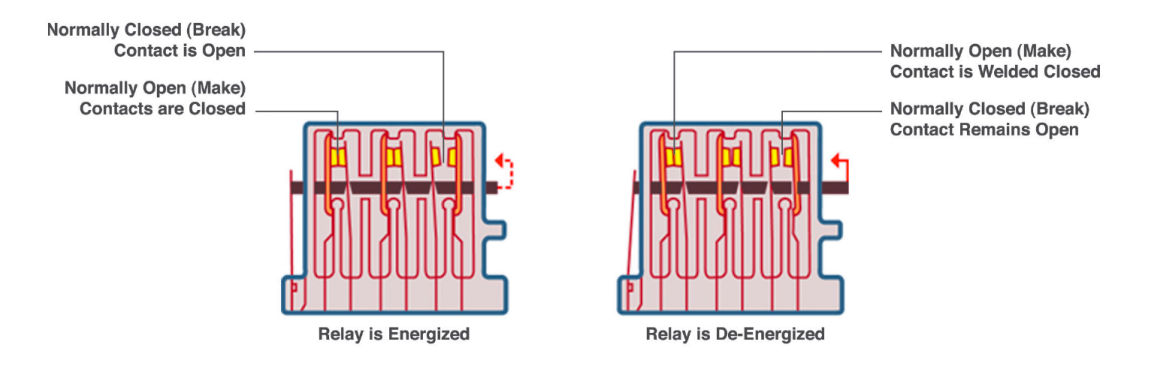
\includegraphics[width = \linewidth]{img/rele_seguridad.png}
    \caption{Funcionamiento de un relé de seguridad \cite{rele_img}}
    \label{fig:rele_seguridad}
\end{figure}


El modelo utilizado en este prototipo, el JW2SN-DC5V es un relé de uso general, pero se optó por reemplazar el relé de seguridad por este modelo de uso general por la gran diferencia que hay en los costos entre los modelos y considerando que el sistema total hace uso de más de 20 relés. \\

Una de las salidas del JW2SN-DC5V se va a utilizar como actuador y la otra para medir el correcto funcionamiento del relé. Para eso, las salidas del contacto secundario van a estar conectadas una a tierra y la otra a una tensión de 3,3 V y la llave secundaria que conmuta va a estar conectada a una entrada digital del MCU para medir el estado de esa llave. A partir de este estado, el sistema puede determinar luego si hay un estado de error y debe tomar medidas para llevar el sistema a un estado seguro. \\


Para poder energizar el relé con una corriente de poco más de 100 mA es necesario utilizar un \textit{driver} de potencia, ya que la corriente es demasiada alta para drivear directamente desde el MCU además de que la tensión de activación es de 5 V y el MCU tiene salidas digitales de 3,3 V. Considerando que el sistema contempla cinco SIS y cada uno tiene dos llaves interruptoras de posible aislamiento, se diseñó un circuito que contemple un mismo \textit{driver} de potencia para múltiples señales. \\

Se eligió el circuito integrado ULN2003D1013TR de STMicroelectronics \cite{ULN2003D1013TR}. Este CI contiene 7 \textit{drivers} NPN Darlington \cite{darlington} donde cada uno puede manejar hasta 500 mA y soportar tensiones de 50 V. Incluye diodos para cargas inductivas lo que lo hace ideal para controlar relés. Para el aislamiento de los SIS, se van a utilizar 2 ULN2003 para manejar los diez relés de aislamiento. \\

En la figura \ref{fig:sis_aislamiento}, se observa el esquemático del \textit{driver} de potencia ULN2003 y un relé con su salida primaria conectada a los terminales del SIS y la salida secundaria a un pin de entrada del MCU. También se observa que se agregó un LED sobre las entradas de la bobina del relé; esto sirve para identificar el estado del relé durante las pruebas. 



\begin{figure}[H]
    \centering
    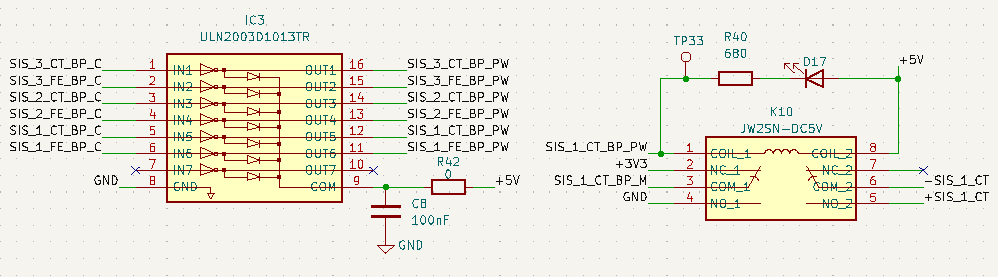
\includegraphics[width = \linewidth]{img/sis_aislamiento.png}
    \caption{Esquemático del circuito de aislamiento de un SIS}
    \label{fig:sis_aislamiento}
\end{figure}


